%!TEX root=../../thesis_rui_almeida.tex
\section{The Experiment}%
\label{sec:the_experiment}

As stated in this chapter's introductory notes, this thesis main body of
work revolves around two base assumptions, our hypothesis. The first
one, about the information capturing by the idealised system, was
addressed in Subsection~\ref{sub:discretisation}. The second, more
physical in nature, is the subject matter of this section. Our
hypothesis states that the light absorption between points $A$ and $B$
(let's call it $A_{AB}$) should be equal to the difference of the
absorptions in $A$ and $B$. We can write this, in a \emph{Lambertian}
manner as in Equation~\ref{eq:lambertian_hypothesis}.

\begin{equation}
    \label{eq:lambertian_hypothesis}
    I_B = I_A \cdot \exp \bigg[-AB \cdot \sum_i \sigma_{ABi} \cdot
    c_{ABi}\bigg]
\end{equation}

This is to say that the light intensity reaching point $B$ is given by
the intensity reaching $A$, exponentially decreased by the absorbers at
interval $AB$. The intensities at $A$ and $B$ are written as in
Equation~\ref{eq:intensityAtAAndB}.

\begin{equation}
    \begin{aligned}
        \label{eq:intensityAtAAndB}
        I_B = I_0 \cdot \exp \bigg[ -L_B \cdot \sum_i \sigma_{Bi} \cdot
        c_{Bi} \bigg]\\
        I_A = I_0 \cdot \exp \bigg[ -L_A \cdot \sum_i \sigma_{Ai} \cdot
        c_{Ai} \bigg]
    \end{aligned}
\end{equation}

If we join all this information in the same expression, the equation is
transformed into its final form, presented in
Equation~\ref{eq:hypothesis_final_form}.

\begin{equation}
    \small
    \label{eq:hypothesis_final_form}
    I_0 \cdot \exp \bigg[ -L_B \cdot \sum_i \sigma_{Bi} \cdot
            c_{Bi} \bigg] = I_0 \cdot \exp \bigg[ -L_A \cdot \sum_i \sigma_{Ai} \cdot
            c_{Ai} \bigg] \cdot \bigg[-AB \cdot \sum_i \sigma_{ABi} \cdot
            c_{ABi}\bigg]
\end{equation}

Equation~\ref{eq:hypothesis_final_form} can be greatly simplified: we
take the natural logarithm of both sides and we state that $\sum_i
\sigma_{Xi} \cdot c_{Xi} = S_i$. These operations result in the
simplified form of Equation~\ref{eq:final_form_simplified}.

\begin{equation}
    \label{eq:final_form_simplified}
    L_B \cdot S_B = L_A \cdot S_A + L_{AB} \cdot S_{AB}
\end{equation}

Now, $L_X \cdot S_X$ can be thought of as the wavelength dependent light
absorption in path $X$. In this case, the wavelength interval is always
the same. We can therefore conclude that, theoretically, our
hypothesis is valid: light absorption between points $A$ and $B$ can be
expressed in terms of the absorption on both these points and
corresponds to their difference.

Although mathematically this seems clear-cut, in the real world things
can become more problematic, since we have to deal with the
imperfections that characterise a real physical system. Noise,
instrumental limitations, adverse environmental effects, etc.. The
experiment we describe in the next few paragraphs aimed at determining
target trace gas concentration in a set analysis field. This field is
dimension-wise compatible with those that would be employed in the final
working system. This experiment is represented in
Figure~\ref{fig:experiment_map}.

\begin{figure}[htpb]
    \centering
    \includegraphics[width=0.8\linewidth]{img/png/experimentMap.png}
    \caption{Location of observer points for the physical experiment.}
    \label{fig:experiment_map}
\end{figure}

The goal of the experiment was to compare passive and active \gls{DOAS}
measurements performed with a very short time difference between them.
The passive measurement would employ the same acquisition strategy as
the drone is expected to use. This comparison will be used to test our
second hypothesis.

Finding two appropriate experiment sites proved to be the first
difficulty: both telescopes should see sky on the back of the other
telescope. Otherwise, the contribution from the terrain's reflection
would have to be taken into account and the experiment conditions would
be very different from the ones the drone will have. There are not many
site pairs that provide this, and most of the ones that exist are
private and authorisations are not easy to obtain. In the end, we
managed to run the experiment in the facilities of \emph{\gls{iep}} and
the \emph{Cristo-Rei} sanctuary, near our own base. 

\subsection{Protocol and conduction}%
\label{sub:protocol_and_conduction}

The experiment involved two different optical assemblies, which are
summarised in Table~\ref{tab:assemblies}. Both assemblies play two
roles, which reflect the comparison between active and passive that is
the entire aim of the test. 

\todo[inline]{Describe artificial light setup and volunteer usage here}

As material in Table~\ref{tab:assemblies} might imply, the East bank
assembly acts as the emitter for the active mode experiment, while the
West bank only plays the part of receiver.

\begin{figure}[htpb]
    \centering
    \caption{Summary table for the two experiment assemblies. Note the
    difference in terms of material, due to the two different roles both
    assemblies play during the experiment.}
    \label{tab:assemblies}
    \missingfigure{}
\end{figure}

The experiment itself is scheduled to start at around 06:00 A.M.. It
consists in capturing spectral measurements in both modes (active and
passive) periodically, with the least amount of time possible between
measurements in the same capture. In this case, I am calling capture to
a particular group of actions that are defined in
Table~\ref{tab:actions}. Captures are defined according to the time at
which they are run, and are summarised in Table~\ref{tab:captures}.
Closing time for this experiment was set on 11:00 A.M.. This time window
ensures measurements are taken during sunrise and until after the
morning rush hour is over.

\begin{table}[htpb]
    \centering
    \small
    \caption{Actions are the indivisible unit upon which each capture is
    built. The prescribed actions for this experiment are described in
    this table.}
    \label{tab:actions}
    \begin{tabularx}{\textwidth}{cXX}
        \toprule
        \textbf{Action ID} & \textbf{Action} & \textbf{Description} \\ \midrule
        A & Active trace gas concentration determination & With the two
        telescopes facing each other, we collect spectra for two minutes
        with the light source turned off and another 2 min with the light
        source turned on. \\
        \midrule
        B & Passive trace gas concentration determination & With the two
        telescopes aligned and approximately facing West, we collect spectra
        for 2 minutes. \\
        \midrule
        C & Passive reference collection & The West telescope points upwards
        and collects data for 2 minutes. \\ \bottomrule
    \end{tabularx}
\end{table}

\begin{table}[htpb]
    \centering
    \caption{Captures are particular sets of actions that are conducted
    according to a specific order, depending on the time of day on which
    the capture is run. This table describes the prescribed captures on
    which this experiment consisted.}
    \label{tab:captures}
    \begin{tabular}{@{}ccc@{}}
        \toprule
        \textbf{Time Frame} & \textbf{Period} & \textbf{Action} \\
        \midrule
        05:00 - Sunrise & 15 minutes & A \\
        Sunrise & Once & C \\
        Sunrise - 11:00 & 15 minutes & A and B\\
        \bottomrule
    \end{tabular}
\end{table}

As displayed in Table~\ref{tab:assemblies}, the spectrometers are both
the same model, manufactured by Avantes and with 2048 channels, powered
through the same \gls{usb} cable that is used for data transfer. The
spectra are acquired through Avantes' own collection software, AvaSoft
8. The spectrometer are configured to have an integration time of 20ms
and immediately store every measurement on an \gls{ascii} file. With the
kind of lighting conditions that we are dealing with, this integration
time allows us not to worry about saturation. However, to build usable
spectra we need to sum the collected files. This is valid because given
the very little time it takes to make a measurement (2 minutes), the sun
can be considered a constant light source, and therefore
we can consider the photons to have a Poissonian statistic
distribution~\cite{Fox2006}.

\subsection{First Run}%
\label{sub:experiment_first_run}

The first attempt at running this experiment took place on June
7\textsuperscript{th} 2021. Weather conditions were optimal for this
kind of measurement, with no wind, clear sky and very low optical
density. The experiment started with a small delay, caused by a problem
on the charger of the East bank laptop. Besides this delay, this was not
a problem for the experiment itself. It was the other laptop's battery
that did not hold enough charge for the experiment to reach its
determined end, and there was no means to charge it on \gls{iep}'s roof.
Given this circumstance, we were able to retrieve spectral measurements
from around 06:20 A.M. to 08:20 A.M., in a total of 6 measurements which
are produced in Table~\ref{tab:experiment_measurements}.

\begin{table}[htpb]
    \centering
    \caption{First run: measurement table.}
    \label{tab:experiment_measurements}
    \resizebox{\textwidth}{!}{%
        \begin{tabular}{@{}lllll@{}}
            \toprule
            \textbf{\#} & \textbf{Passive meas.} & \textbf{Passive ref.} & \textbf{Active mean.} & \textbf{Active ref.} \\ \midrule
            1 & 06:20 & 06:23 & 06:15 & -- \\
            2 & 06:46 & 06:50 & 06:41 & -- \\
            3 & 07:04 & 07:07 & 07:00 & -- \\
            4 & 07:25 & 07:27 & 07:21 & -- \\
            5 & 07:48 & 07:50 & 07:45 & -- \\
            6 & 08:10 & 08:12 & 08:06 & 08:08 \\ \bottomrule
        \end{tabular}%
    }
\end{table}

On the one hand, it is clear from
Table~\ref{tab:experiment_measurements} that we do not have data on the
active baseline spectra~\footnote{In this case, the baseline spectrum is
one taken in the exact same direction and approximately
simultaneously, with the light turned off to allow removal of solar
contribution.} (likely due to some operation error); on the other hand,
we have too few data points to make any claim of validation or
refutation of the principle we were to measure. It was thus clear that
another run was necessary to get the necessary results.

Although it was not possible to produce convincing results from these
data, they were of good individual quality and allowed some preliminary
analysis to be run. Using the first measurement as the reference
spectrum, it was possible to calculate optical densities for each one of
the measurement moments, as well as \gls{no2} concentration. The
graphical appearance of the optical density signal for each measurement
is presented in Figure~\ref{fig:active_optical_densities} and
Figure~\ref{fig:passive_optical_densities}, while the concentration
chart for the various moments comprises
Figure~\ref{fig:calculated_concentration}.

\begin{figure}[htpb]
    \centering
    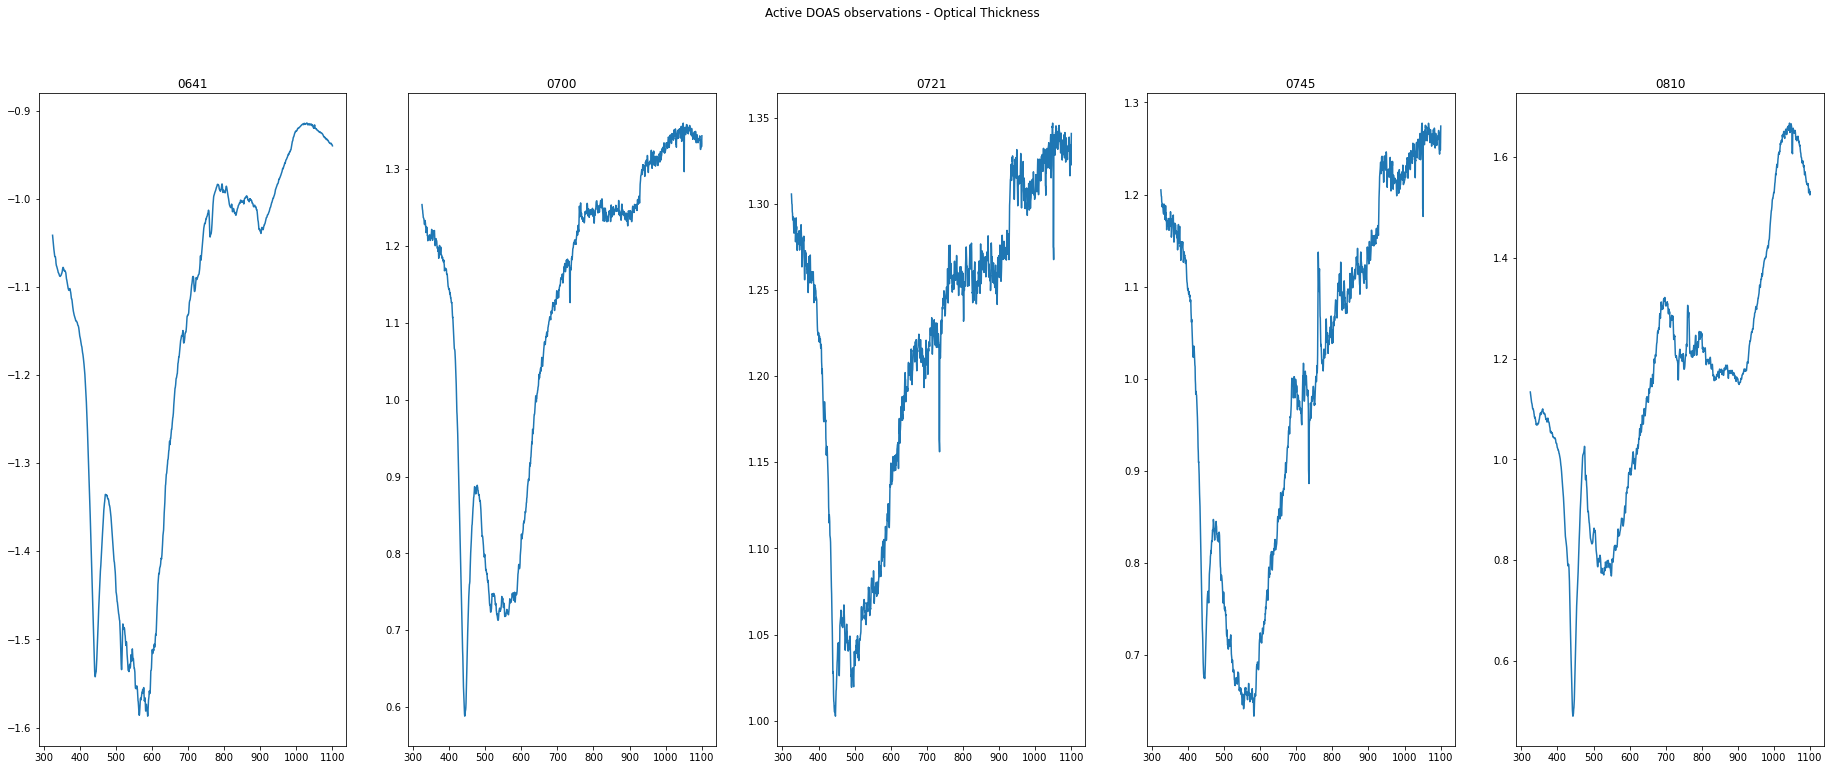
\includegraphics[width=0.8\linewidth]{img/png/tau_activeDOAS.png}
    \caption{Optical densities calculated with reference to measurement
    \#1 for the other measurement moments in the active DOAS mode.} 
    \label{fig:active_optical_densities}
\end{figure}

\begin{figure}[htpb]
    \centering
    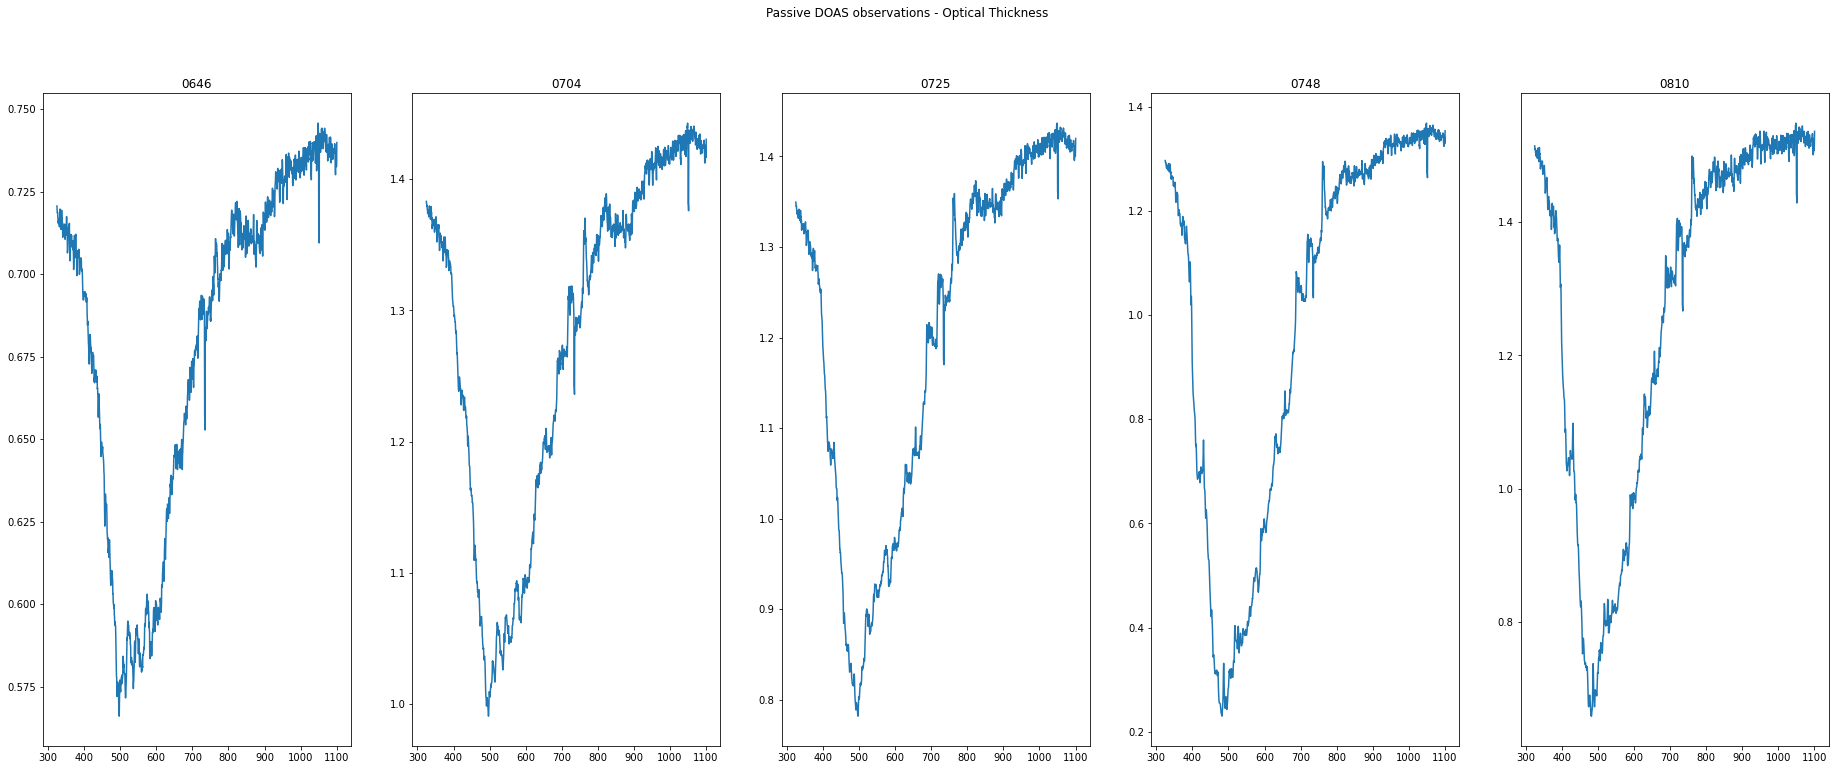
\includegraphics[width=0.8\linewidth]{img/png/tau_passiveDOAS.png}
    \caption{Optical densities calculated with reference to measurement
    \#1 for the other measurement moments in the passive DOAS mode.} 
    \label{fig:passive_optical_densities}
\end{figure}

\begin{figure}[htpb]
    \centering
    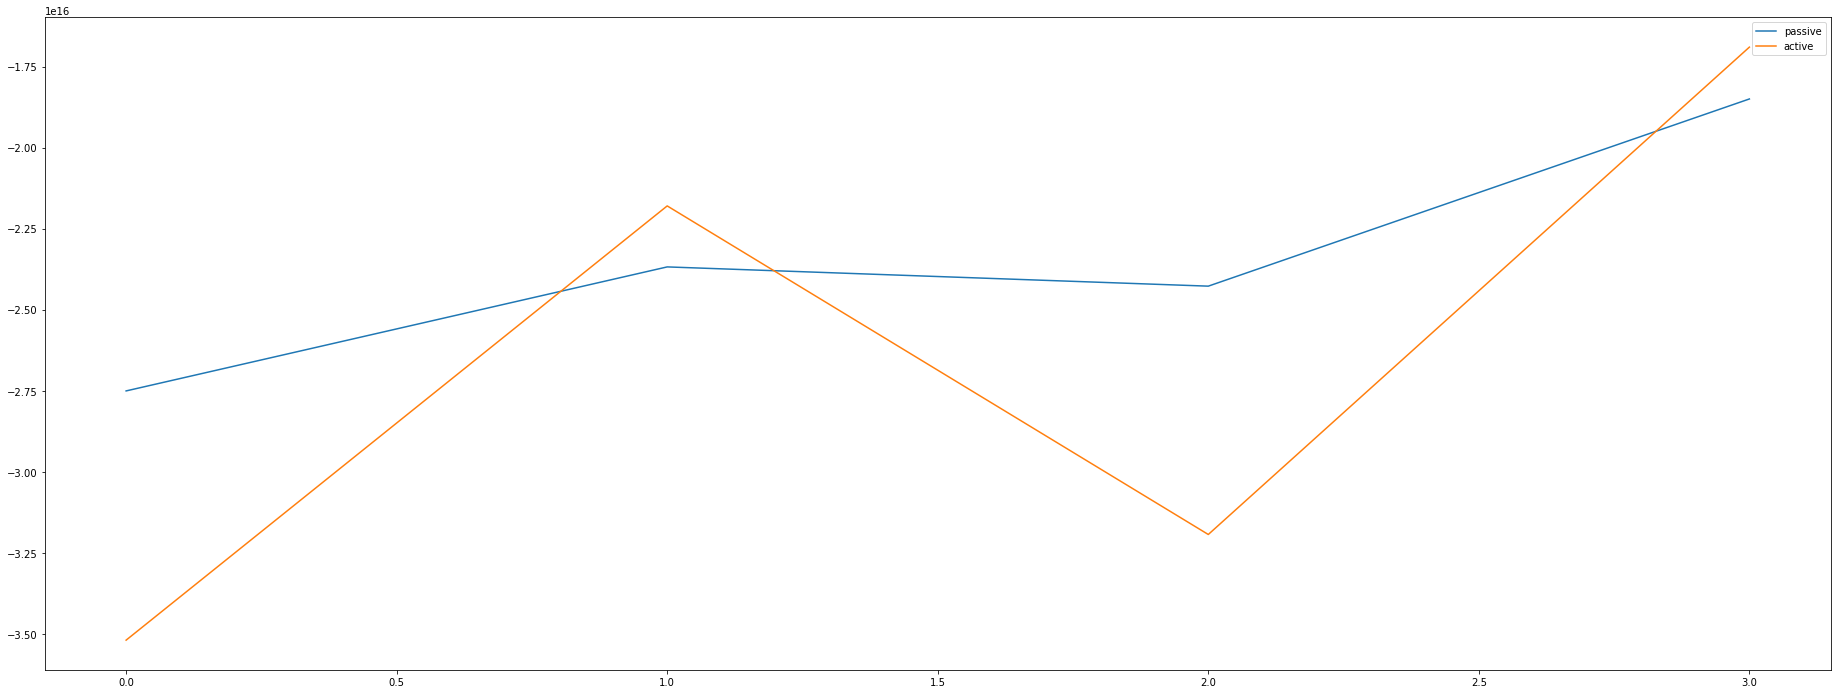
\includegraphics[width=0.8\linewidth]{img/png/calculatedConcentrations.png}
    \caption{Calculated \gls{no2} concentrations for the various
    measurement moments. Each integer in the horizontal axis corresponds
    to a moment, organized chronologically.}
    \label{fig:calculated_concentration}
\end{figure}

Although admittedly incomplete, these data allows some preliminary
remarks. The first and most important one is that the highest
concentration detected appears in the first measurement point for both
active and passive modes. The passive mode measurement could be
discarded because this measurement was taken during sunrise and the
relevant spectra could be considered too noisy. However, its active
counterpart produces the exact same result, as the chart in
Figure~\ref{fig:calculated_concentration} shows. The second data point
had the lowest detected concentration, and from that point forward, the
concentration evolves as expected (rising). One other remark that could
be addressed towards this first stage analysis is that there seems to be
a good agreement between active and passive measurements. This remark
might be considered invalid, as there is no data for the active
baseline. However, since this analysis was focused on \gls{no2}
concentration, and the relevant spectral window for this trace gas is
usually between 400nm and 500nm, this is not the case. In effect, the
scattered-sunlight-originated photon counts in this interval will be
always much smaller than the artificial ones, thus having an
equivalently smaller influence in the final results. 

\subsection{Second run}%
\label{sub:second_run}


\subsection{Data Processing}%
\label{sub:data_processing}


